\documentclass[a4paper,11.5pt]{article}
\usepackage[textwidth=170mm, textheight=230mm, inner=20mm, top=20mm, bottom=30mm]{geometry}
\usepackage[normalem]{ulem}
\usepackage[utf8]{inputenc}
\usepackage[T1]{fontenc}
\PassOptionsToPackage{defaults=hu-min}{magyar.ldf}
\usepackage[magyar]{babel}
\usepackage{amsmath, amsthm,amssymb,paralist,array, ellipsis, graphicx,float,framed}
%\usepackage{marvosym}
\makeatletter
\renewcommand*{\mathellipsis}{%
	\mathinner{%
		\kern\ellipsisbeforegap%
		{\ldotp}\kern\ellipsisgap%
		{\ldotp}\kern\ellipsisgap%
		{\ldotp}\kern\ellipsisaftergap%
	}%
}
\renewcommand*{\dotsb@}{%
	\mathinner{%
		\kern\ellipsisbeforegap%
		{\cdotp}\kern\ellipsisgap%
		{\cdotp}\kern\ellipsisgap%
		{\cdotp}\kern\ellipsisaftergap%
	}%
}
\renewcommand*{\@cdots}{%
	\mathinner{%
		\kern\ellipsisbeforegap%
		{\cdotp}\kern\ellipsisgap%
		{\cdotp}\kern\ellipsisgap%
		{\cdotp}\kern\ellipsisaftergap%
	}%
}
\renewcommand*{\ellipsis@default}{%
	\ellipsis@before
	\kern\ellipsisbeforegap
	.\kern\ellipsisgap
	.\kern\ellipsisgap
	.\kern\ellipsisgap
	\ellipsis@after\relax}
\renewcommand*{\ellipsis@centered}{%
	\ellipsis@before
	\kern\ellipsisbeforegap
	.\kern\ellipsisgap
	.\kern\ellipsisgap
	.\kern\ellipsisaftergap
	\ellipsis@after\relax}
\AtBeginDocument{%
	\DeclareRobustCommand*{\dots}{%
		\ifmmode\@xp\mdots@\else\@xp\textellipsis\fi}}
\def\ellipsisgap{.1em}
\def\ellipsisbeforegap{.05em}
\def\ellipsisaftergap{.05em}
\makeatother

\usepackage{hyperref}
\hypersetup{
	colorlinks = true	
}

\DeclareMathOperator{\Int}{int}
\DeclareMathOperator{\tg}{tg}
\DeclareMathOperator{\ctg}{ctg}
\DeclareMathOperator{\Th}{th}
\DeclareMathOperator{\sh}{sh}
\DeclareMathOperator{\ch}{ch}
\DeclareMathOperator{\sgn}{sgn}
\DeclareMathOperator{\arc}{arc}
\DeclareMathOperator{\arctg}{arc tg}
\DeclareMathOperator{\arcctg}{arc ctg}

\begin{document}
	%%%%%%%%%%%RÖVIDÍTÉSEK%%%%%%%%%%
	\setlength\parindent{0pt}
	\def\s{\hspace{0.2mm}\vphantom{\beta}}
	\def\Z{\mathbb{Z}}
	\def\Q{\mathbb{Q}}
	\def\R{\mathbb{R}}
	\def\C{\mathbb{C}}
	\def\N{\mathbb{N}}
	\def\Ra{\overline{\mathbb{R}}}
	
	\def\sume{\displaystyle\sum_{n=1}^{+\infty}}
	\def\sumn{\displaystyle\sum_{n=0}^{+\infty}}
	
	\def\narrow{\underset{n\rightarrow+\infty}{\longrightarrow}}
	\def\limn{\displaystyle\lim_{n\to +\infty}}
	\def\limx{\displaystyle\lim_{x\to +\infty}}
	
	\pagestyle{plain}
	\theoremstyle{definition}
	\newtheorem{theorem}{Tétel}[subsection] 
	
	\theoremstyle{definition}
	\newtheorem{definition}[theorem]{Definíció} 
	\newtheorem{example}[theorem]{Példa} 
	\newtheorem{task}[theorem]{Feladat} 
	\newtheorem{note}[theorem]{Megjegyzés}
	\newtheorem{revision}[theorem]{Emlékeztető}
	%%%%%%%%%%%%%%%%%%%%%%%%%%%%%%%%%%%%%%%%%%%%%%%%%%%%%%%%%%%%%%%%%%%%%
	\begin{center}
		{\LARGE\textbf{Analízis II.}}
		\smallskip
		
		{\Large 2. zh tételkidolgozás}
	\end{center}
	A jegyzetet \textsc{Umann} Kristóf készítette Dr. \textsc{Szili} László  előadása alapján. (\today)
	\begin{enumerate}
		\item \textbf{A konvexitás ekvivalens átfogalmazása egyenlőtlenséggel.}
		
		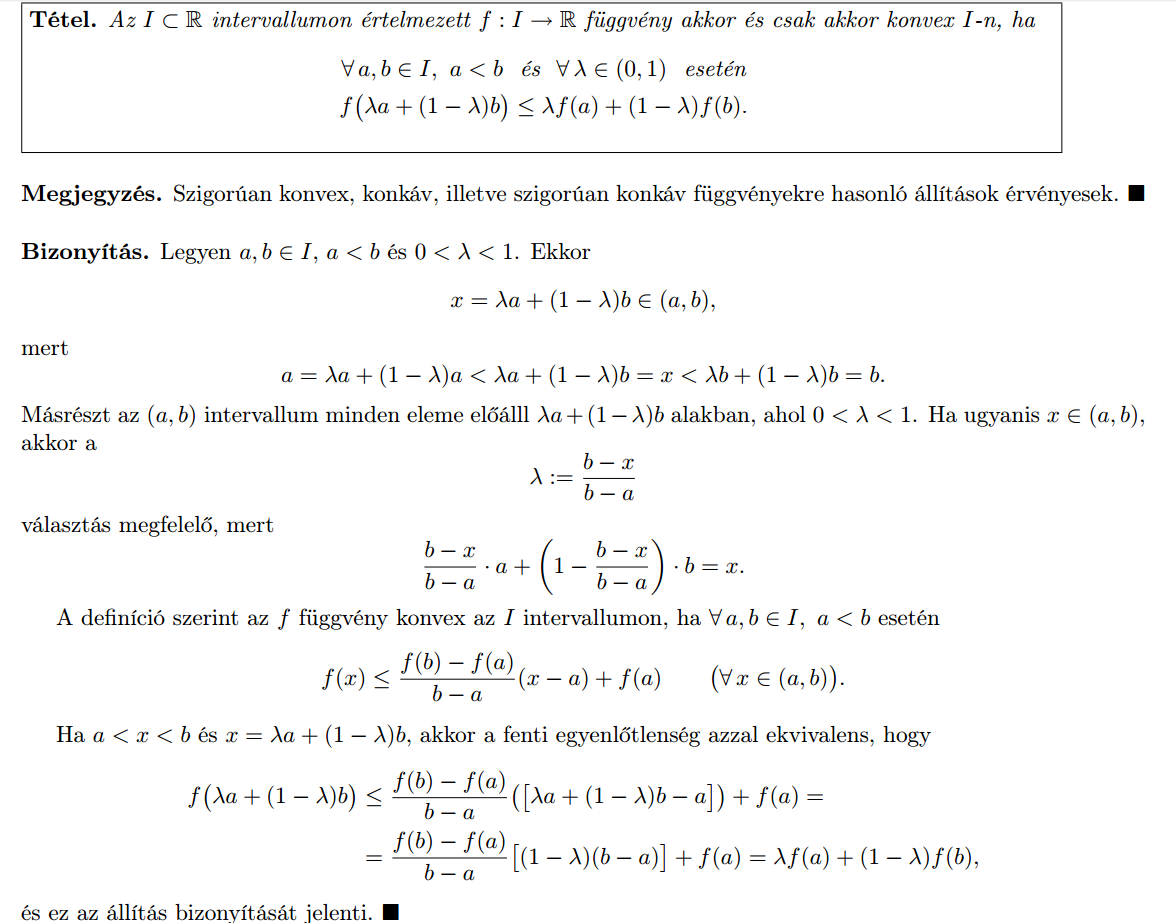
\includegraphics[width = \textwidth]{kepek/01.png}
		
		\item \textbf{A konvexitás jellemzése a deriváltfüggvénnyel.}
		
		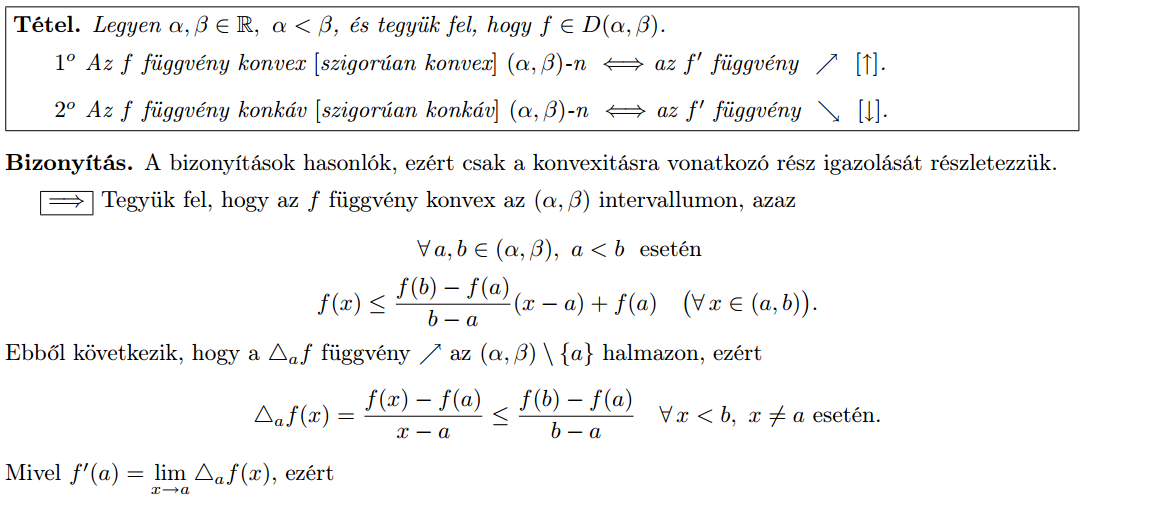
\includegraphics[width = \textwidth]{kepek/02true_1.png}
		
		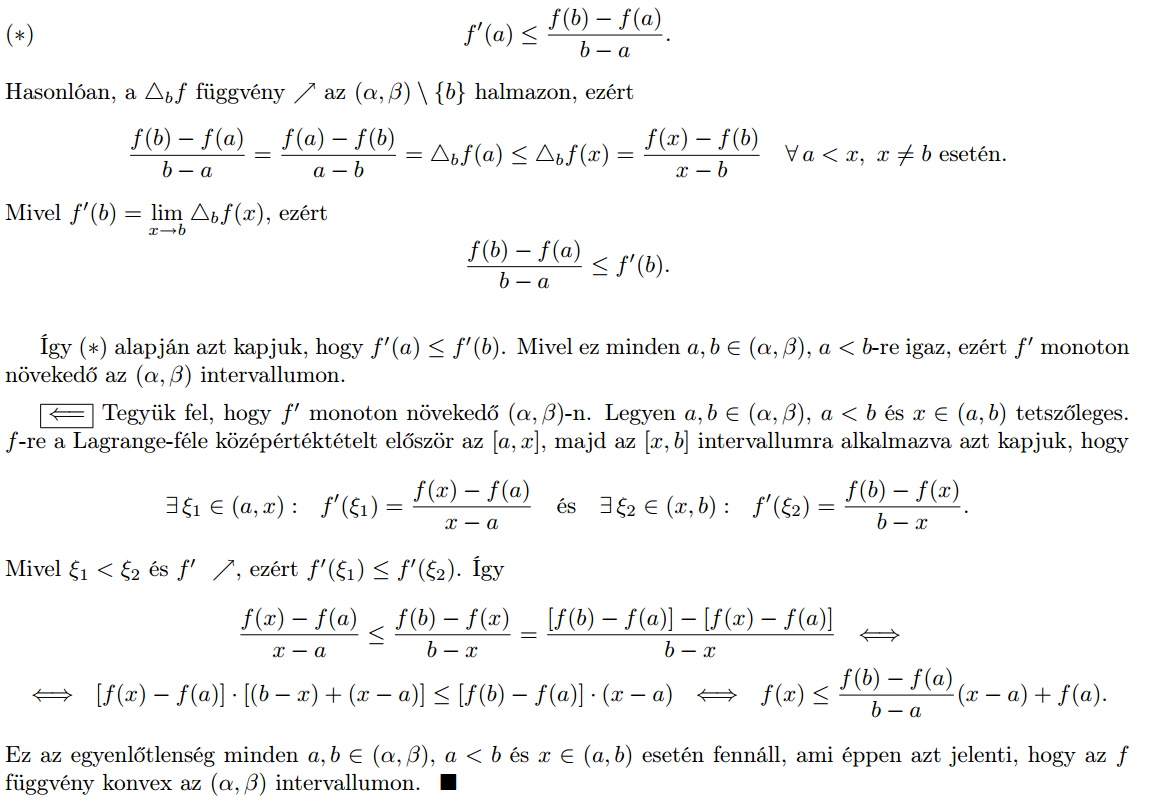
\includegraphics[width = \textwidth]{kepek/02true_2.png}
		
		\item \textbf{A $\pi$ szám bevezetését megalapozó állítás}
		
		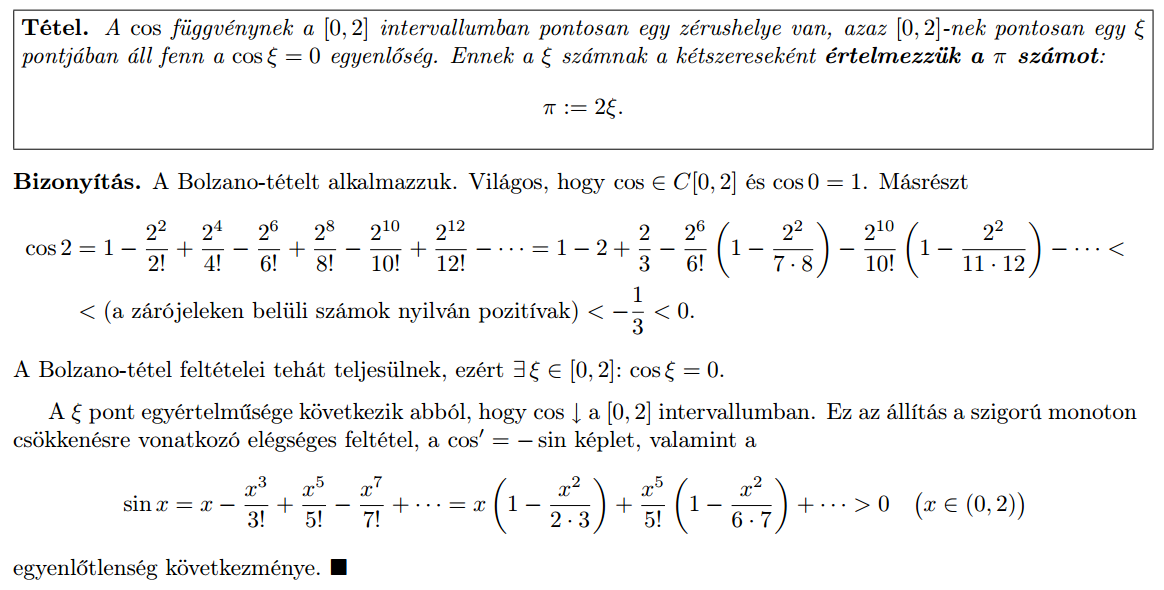
\includegraphics[width = \textwidth]{kepek/03.png}
		\pagebreak
		
		\item \textbf{A $\frac{0}{0}$ esetre vonatkozó L’Hospital-szabály.}
		
		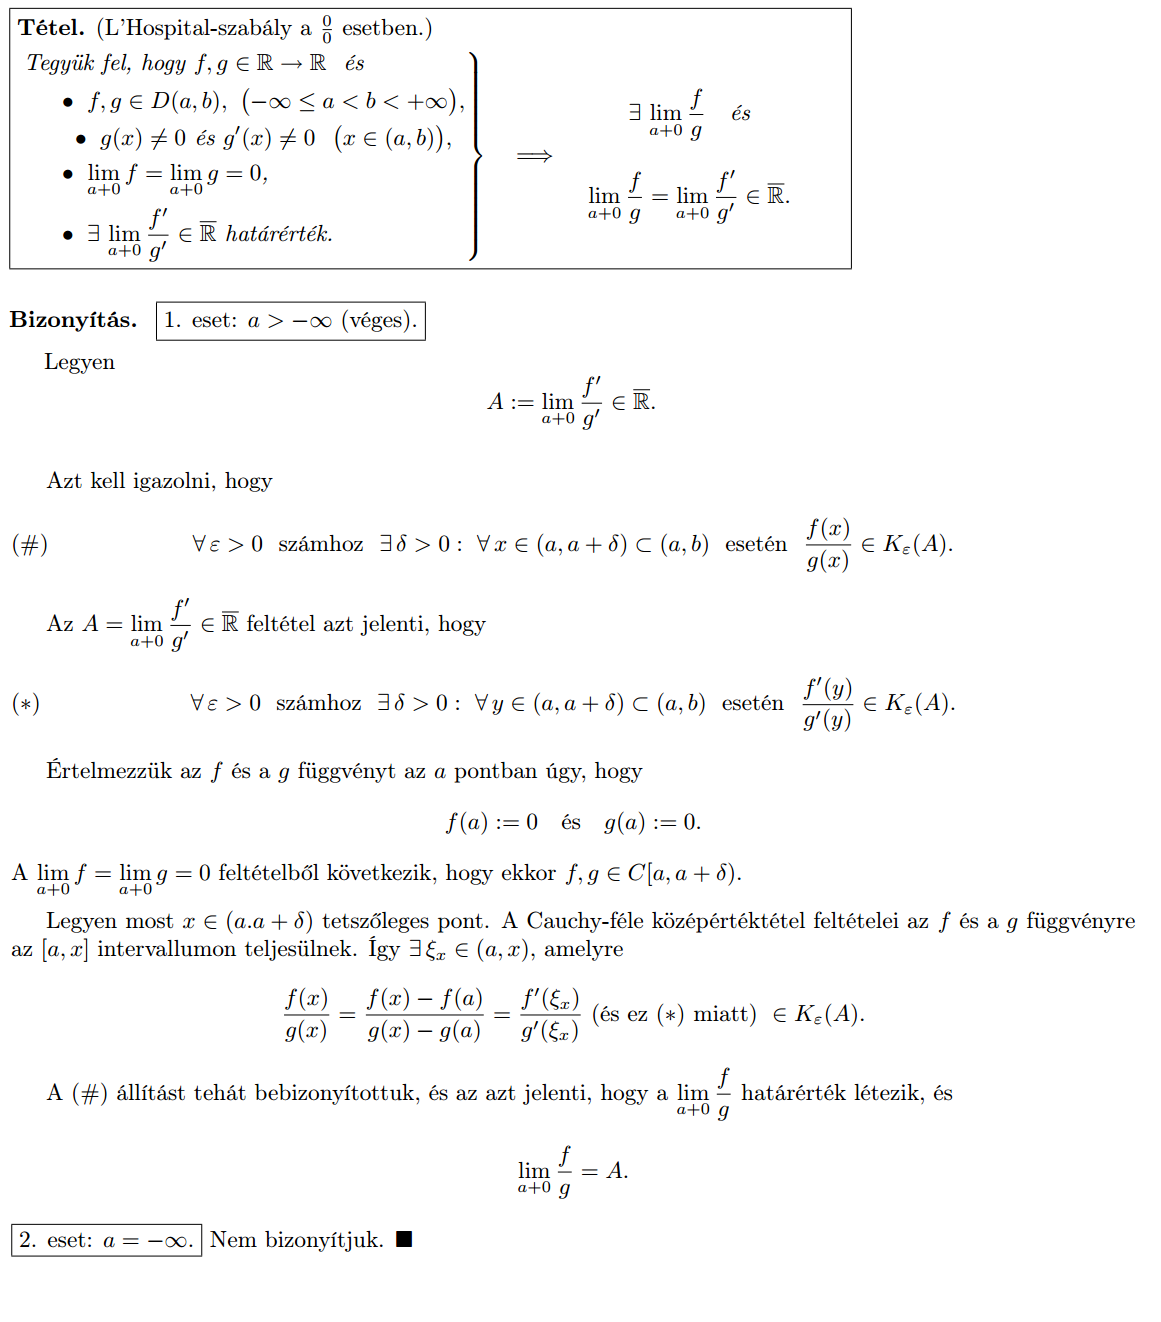
\includegraphics[width = \textwidth]{kepek/04.png}
		
		\item \textbf{A Taylor-formula a Lagrange-féle maradéktaggal.}
		
		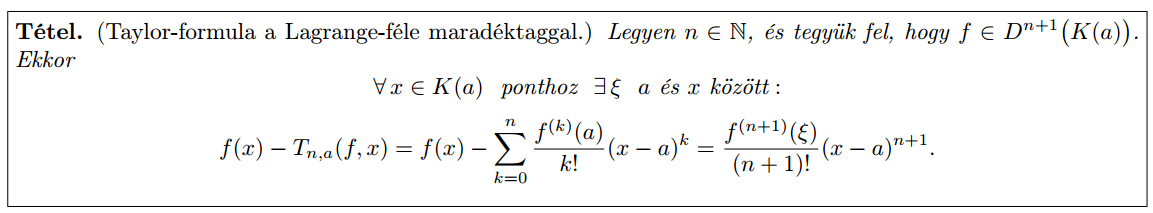
\includegraphics[width = 160mm]{kepek/05_1.png}
		
		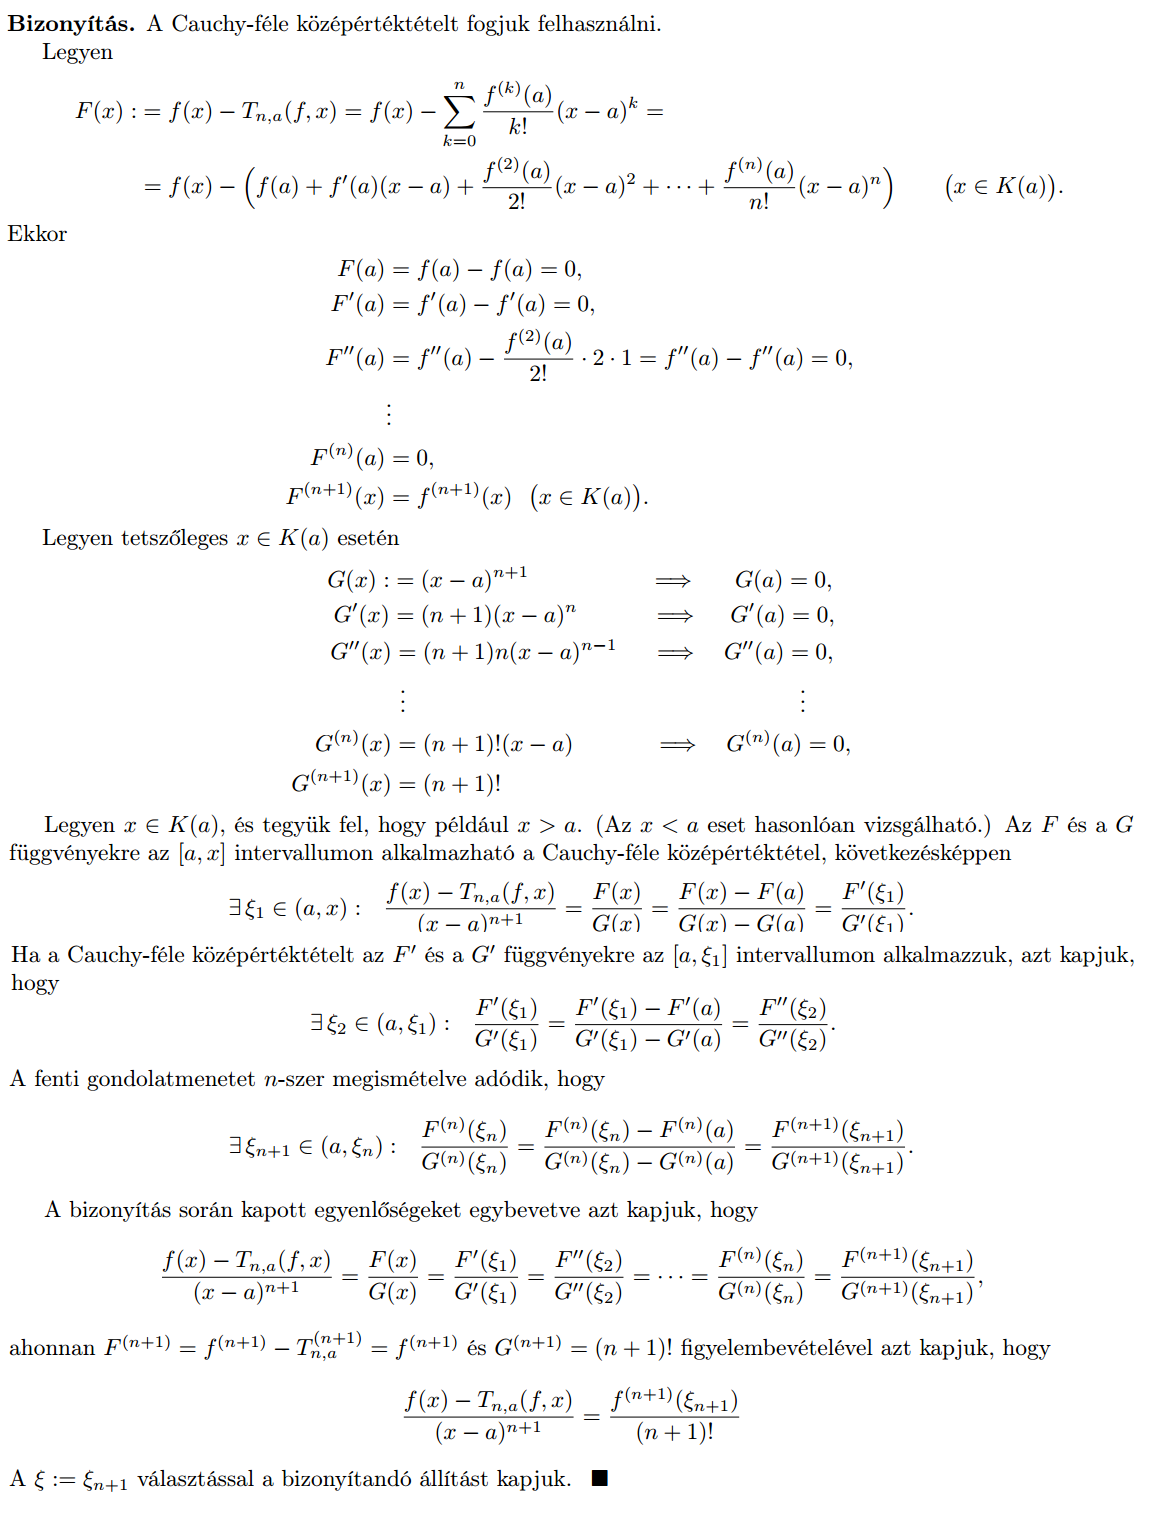
\includegraphics[width = 160mm]{kepek/05_2.png}
		
		\item \textbf{A $\sqrt{1-x^2}\quad  (x\in(-1,1))$ primitív függvényeinek előállítása.}
		\begin{framed}
			\[ \int\sqrt{1-x^2}\, dx = \frac{\arc\sin x+x\sqrt{1-x^2}}{2}+c \quad (x\in(-1,1),\quad c\in\R) \]
		\end{framed}
		\textit{Megoldás:}
		
		Alkalmazzuk az $x=\sin t = g(t)\quad (x\in(-1,1)), \quad t\in\left(-\frac{\pi}{2},\frac{\pi}{2}\right)$ helyettesítést:
		\[ g'(t)=\cos t>0\quad \left(|t|<\frac{\pi}{2}\right)\quad \Rightarrow\quad \exists g^{-1}; \quad t:=\arc\sin x \]
		\[ \int \sqrt{1-x^2}\,dx=\int\underbrace{\sqrt{1-\sin^2t}}_{=\cos t>0}\cdot\cos t\, dt\quad \overset{\cos2t=\cos^2t-\sin^2t}{\underset{\sin^2t+\cos^2t=1}{=}}\quad \int \frac{1+\cos2t}{2}dt= \]
		\[ = \frac{t}{2}+\frac{\sin2t}{4} + c=\frac{t}{2}+\frac{2\sin t\cdot \cos t}{4}+c\big|_{t=\arc\sin x}=\frac{\arc\sin x + x\cdot\cos(\arc\sin x)}{2}+c \]
		\[\cos(\underbrace{\arc\sin x}_{\stackrel{=:\alpha\in\left(-\frac{\pi}{2},\frac{\pi}{2}\right)}{\sin\alpha=x}})=\pm\sqrt{1-\sin^2\alpha}=\sqrt{1-x^2}\]
		\[ \int\sqrt{1-x^2}\,dx=\frac{\arc\sin x+x\sqrt{1-x^2}}{2}+c.\quad (c\in\R)\quad \blacksquare \] 
		
		\item\textbf{Oszcillációs összegek. Az integrálhatóság jellemzése az oszcillációs összegekkel.}
		\begin{framed}
			Tegyük fel, hogy $f[a,b]\to\R$ korlátos függvény. Ekkor:
			\[ f\in R[a,b]\quad \Leftrightarrow\quad \begin{gathered}
			\forall\varepsilon>0\quad \exists\tau\in\mathcal{F}[a,b],\quad  \varOmega(f;\tau)<\varepsilon\\
			\text{(az oszcillációs összeg tetszőlegesen kicsi lehet)}
			\end{gathered} \]
		\end{framed}
		\textit{Bizonyítás:}
		
		\fbox{$\Rightarrow:$}
		\[ I_*(f)=I^*(f)=:I \]
		$\varepsilon>0$ tetszőleges, szuprémum definíciójából:
		\[ \varepsilon>0\text{-hoz}\quad \exists\tau_1\in\mathcal{F}[a,b],\quad I-\frac{\varepsilon}{2}<s(f;\tau_1)\leq I \]
		\[ \varepsilon>0\text{-hoz}\quad \exists\tau_2\in\mathcal{F}[a,b],\quad I<S(f;\tau_2)\leq I+\frac{\varepsilon}{2} \]
		Legyen \fbox{$\tau:=\tau_1\cup\tau_2$}.
		\[ I-\frac{\varepsilon}{2}\ <s(f;\tau_1)\leq\  s(f;\tau)\leq\  S(f;\tau)\leq\  S(f;\tau_2)<\ I+\frac{\varepsilon}{2} \]
		\[ \Rightarrow\quad\varOmega(f;\tau)= S(f;\tau)-s(f;\tau)<\varepsilon. \]
		\fbox{$\Leftarrow:$}
		$\varepsilon>0\text{-hoz}\quad \exists\tau\in\mathcal{F}[a,b]\quad \varOmega(f;\tau)<\varepsilon:$
		\[ \varOmega(f;\tau)=S(f;\tau)-s(f;\tau)\geq I^*(f)-I_*(f)\geq 0 \]
		\[ \Rightarrow\quad 0\leq I^*(f)-I_*(f)<\varepsilon \]
		\[ \Rightarrow\quad I^*(f)-I_*(f)=0\quad \Rightarrow\quad I^*(f)=I_*(f)\Rightarrow\quad f\in R[a,b].\quad \blacksquare \]
		
		\item \textbf{Monoton függvény integrálható.}
		\begin{framed}
			\begin{center}	
				Ha $f\in K[a,b]$ ÉS monoton \quad $\Rightarrow\quad f\in R[a,b].$
			\end{center}
		\end{framed}
		\medskip
		
		\textit{Bizonyítás:} (oszcillációs összegekkel)
		Legyen $f$ (például) $\nearrow [a,b]$-n.
		\[ \tau:=\{ a=x_0<x_1<\ldots<x_n=b \}\in\mathcal{F}[a,b]\quad \text{tetszőleges} \]
		\[ \inf\{ f(x)\ | \ x_i\leq x\leq x_{i+1} \}=:m:=f(x_i) \]
		\[ \sup\{ f(x)\ | \ x_i\leq x\leq x_{i+1} \}=:M:=f(x_{i+1}) \]
		\[ \varOmega(f,\tau)=S(f,\tau)-s(f,\tau)=\sum_{i=0}^{n-1}M_i(x_{i+1}-x_i)-\sum_{i=0}^{n-1}m_i(x_{i+1}-x_i)= \]
		\[ = \sum_{i=0}^{n-1}(M_i-m_i)(x_{i+1}-x_i)=\sum_{i=0}^{n-1}\overbrace{\left(f(x_{i+1})-f(x_i)\right)}^{\geq 0}\overbrace{(x_{i+1}-x_i)}^{\geq 0}\leq \max_{0\leq i\leq n-1}(x_{i+1}-x_i)\cdot\sum_{i=0}^{n-1}(f(x_{i+1})-f(x_i))\]
		\text{-- teleszkópikus!}
		\[ \Rightarrow\quad \varOmega(f,\tau)\leq ||\tau||\cdot (f(b)-f(a)) \]
		\[ \forall\varepsilon>0\quad \tau\in\mathcal{F}[a,b]:\quad ||\tau||<\frac{\varepsilon}{f(b)-f(a)} \]
		\[ \Rightarrow\quad \varOmega(f,\tau)<\varepsilon\quad \Rightarrow\quad f\in R[a,b].\quad \blacksquare \]
		
		\item \textbf{A Newton-Leibniz tétel.}
		\begin{framed}
			Tegyük fel, hogy
			\[ \left.\begin{gathered}
			f\in R[a,b]\\
			f\text{-nek van primitív függvénye}\quad [a,b]\text{-n}\\
			\end{gathered}\right\} \quad \Rightarrow\quad \int_a^bf=F(b)-F(a)=:[F(x)]_a^b  \]
			ahol $F$ az $f$ egy primitív függvénye.
		\end{framed}
		
		\textit{Bizonyítás:} Legyen $\tau:=\{ a=x_0<x_1<\ldots<x_n=b \}\in\mathcal{F}[a,b]$ tetszőleges.
		\[ F(b)-F(a)=F(x_n)-F(x_0)\quad \overset{\text{TRÜKK}}{=}\quad \big(F(x_n)-F(x_{n-1})\big)+\big(F(x_{n-1})-F(x_{n-2})\big)+\ldots+\big(F(x_1)-F(x_0)\big)=\]
		\[=\sum_{i=0}^{n-1}F(x_{i+1})-F(x_i)= \]
		Tegyünk egy apróbb megállapítást: $F$-re $[x_i,x_{i+1}]$-en a Lagrange középérték tétel: 
		\[ F(x_{i+1})-F(x_i)=F'(\xi_i)(x_{i+1}-x_i)\quad \overset{F'=f}{=}\quad f(\xi_i)(x_{i+1}-x_i) \]
		Folytatván a bizonyítást:
		\[ F(b)-F(a)=\sum_{i=0}^{n-1}f(\xi_i)(x_{i+1}-x_i) \]
		\[ \Downarrow \]
		\[ s(f,\tau)\leq F(b)-F(a)\leq S(f,\tau)\quad \inf\]
		$\forall \tau$-ra $\sup\quad \Rightarrow\quad $
		\[ I_*(f)\leq F(b)-F(a)\leq I^*(f) \]
		\[ f\in R[a,b]\quad \Rightarrow\quad I_*(f)=I^*(f)=\int_a^bf=\int_a^bf=F(b)-F(a).\quad \blacksquare \]
		\pagebreak
		\item \textbf{Az integrálfüggvény folytonosságára vonatkozó állítás.}
		\begin{framed}
			Tegyük fel hogy $f\in R[a,b],\quad x_0\in[a,b],$
			\[ F(x):=\int_{x_0}^xf(t)\,dt\quad (x\in[a,b]). \]
			Ekkor az $F$ függvény folytonos $[a,b]$-n.
		\end{framed}
		\textit{Bizonyítás:} $c\in[a,b]$ tetszőleges, \quad $x\in[a,b],\quad $ és pl. $x>c.$
		\[ |F(x)-F(c)|=\left|\int_{x_0 }^xf-\int_{x_0}^cf\right|=\left|\int_{x_0 }^xf+\int^{x_0}_cf\right|=\left|\int_{c}^xf(t)\,dt\right|\quad \overset{x>0}{\leq}\quad \int_{c}^x|f(t)|\,dt\leq\]
		\[\overset{M:=\underset{[a,b]}{\sup}|f|<+\infty}{\leq}\quad M\cdot\int_{c}^x1\,dt=M|x-c|  \]
		\[ 0\leq|F(x)-F(c)|\leq M|x-c|\quad  \Rightarrow\quad \lim_{x\to c}|F(x)-F(c)|=0\quad \Rightarrow\quad \lim_{x\to c}F(x)-F(c)=0\]\[\Rightarrow\quad \lim_{x\to c}F(x)=F(c)\quad \Rightarrow\quad F\in C\{c\}\quad \overset{\text{$c$ tetszőleges}}{\Rightarrow}\quad F\in C[a,b].\quad \blacksquare \]
		\item \textbf{Az integrálfüggvény differenciálhatóságára vonatkozó állítás.}
		\begin{framed}
			Tegyük fel hogy $f\in R[a,b],\quad x_0\in[a,b],$
			\[ F(x):=\int_{x_0}^xf(t)\,dt\quad (x\in[a,b]). \]
			Ha $f\in C\{d\}\quad (d\in(a,b)),$ akkor az $F\in D\{d\}$ és $F'(d)=f(d)$.
		\end{framed}
		\textit{Bizonyítás:} Tegyük fel hogy $d\in(a,b)$ és $f\in C{\{d\}}.$
		
		Igazoljuk:
		\[ F\in D\{d\} \quad \text{és}\quad f(d)=F'(d):=\lim_{h\to0}\frac{F(d+h)-F(d)}{h} \]
		\[ \Leftrightarrow\quad \lim_{h\to0}\left(f(d)-\frac{F(d+h)-F(d)}{h}\right)=0\quad \Leftrightarrow\quad \lim_{h\to0}\left|f(d)-\frac{F(d+h)-F(d)}{h}\right|=0, \]
		azaz \quad $\displaystyle\forall\varepsilon>0\quad \exists\delta>0\quad \forall|h|<\delta:\quad \left|f(d)-\frac{F(d+h)-F(d)}{h}\right|<\varepsilon.\quad  (*)$
		
		\smallskip
		Legyen $\varepsilon>0$ adott:
		\[ \left|f(d)-\frac{F(d+h)-F(d)}{h}\right|=\left|f(d)-\frac{1}{h}\left(\int_{x_0}^{d+h}f-\int_{x_0}^{d}f\right)\right|=\left|f(d)-\frac{1}{h}\left(\int_{x_0}^{d+h}f+\int_{d}^{x_0}f\right)\right|=\]
		\[\left|f(d)-\frac{1}{h}\int_{d}^{d+h}f(t)\,dt\right| \quad  \overset{f(d)=\frac{1}{h}\int_{d}^{d+h}f(d)\,dt}{=}\quad \left|\frac{1}{h}\int_{d}^{d+h}f(d)-f(t)\,dt\right|\quad \overset{h>0}{\leq}\quad \frac{1}{h}\int_d^{d+h}|f(d)-f(t)|\,dt. \]
		Mivel $f\in C\{d\}\quad \Rightarrow\quad \varepsilon$-hoz$\quad \exists\delta>0\quad \forall|t-d|<\delta:\quad |f(d)-f(t)|<\varepsilon$.
		
		\smallskip
		Ha $h>0,\quad (0<h<\delta)$ és $t\in[d,d+h]\quad \Rightarrow$
		\[ \left|f(d)-\frac{F(d+h)-F(d)}{h}\right|\leq\frac{1}{h}\cdot\varepsilon\underbrace{\int_d^{d+h}1\,dt}_{=h}=\varepsilon\quad \Rightarrow\quad (*).\quad \blacksquare \]
	\end{enumerate}
\end{document}